% Fig 1: NeuroPLC End-to-End Pipeline (fixed: balanced density, prominent numbers, clear annotations)
\documentclass[tikz,border=10pt]{standalone}
\usepackage{tikz}
\usepackage{fontspec}
\usetikzlibrary{shapes.geometric, arrows.meta, positioning, calc, fit, backgrounds, shadows}

\definecolor{steel}{HTML}{2563eb}
\definecolor{teal}{HTML}{0d9488}
\definecolor{amber}{HTML}{d97706}
\definecolor{purple}{HTML}{7c3aed}
\definecolor{rose}{HTML}{e11d48}
\definecolor{ink}{HTML}{1e293b}
\definecolor{slate}{HTML}{64748b}
\definecolor{graybg}{HTML}{f1f5f9}

\begin{document}
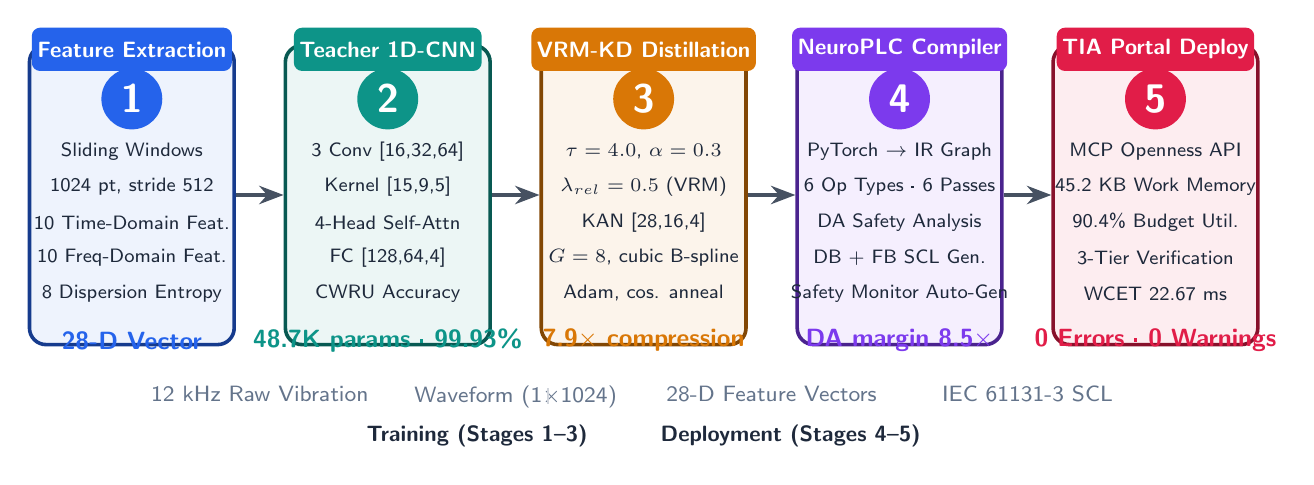
\begin{tikzpicture}[
    stage/.style={
        rectangle, rounded corners=6pt,
        draw=#1!60!black, fill=#1!08, line width=1.3pt,
        text=ink, minimum width=2.6cm, minimum height=3.8cm,
        font=\sffamily, align=center, inner sep=4pt,
    },
    titlebar/.style={
        rectangle, rounded corners=3pt,
        fill=#1, text=white,
        font=\sffamily\footnotesize\bfseries, align=center,
        minimum width=2.35cm, minimum height=0.55cm, inner sep=2pt,
    },
    arr/.style={
        -{Stealth[scale=0.9]}, line width=1.5pt, slate!70!black,
    },
    badge/.style={
        circle, fill=#1, text=white,
        font=\sffamily\Large\bfseries,
        minimum size=22pt, inner sep=0pt,
    },
    detail/.style={
        font=\sffamily\scriptsize, text=ink, align=center, inner sep=0.5pt,
    },
    keymetric/.style={
        font=\sffamily\small\bfseries, text=#1,
    },
]

% x positions evenly spaced
\def\dx{3.25}

% ── Stage 1: Feature Extraction ──
\node[stage=steel] (S1) at (0,0) {};
\node[titlebar=steel] at (0,1.85) {Feature Extraction};
\node[badge=steel] at (0,1.22) {1};
\node[detail] at (0,0.55) {Sliding Windows};
\node[detail] at (0,0.10) {1024 pt, stride 512};
\node[detail] at (0,-0.35) {10 Time-Domain Feat.};
\node[detail] at (0,-0.80) {10 Freq-Domain Feat.};
\node[detail] at (0,-1.25) {8 Dispersion Entropy};
\node[keymetric=steel] at (0,-1.85) {28-D Vector};

% ── Stage 2: Teacher CNN ──
\node[stage=teal] (S2) at (\dx,0) {};
\node[titlebar=teal] at (\dx,1.85) {Teacher 1D-CNN};
\node[badge=teal] at (\dx,1.22) {2};
\node[detail] at (\dx,0.55) {3 Conv [16,32,64]};
\node[detail] at (\dx,0.10) {Kernel [15,9,5]};
\node[detail] at (\dx,-0.35) {4-Head Self-Attn};
\node[detail] at (\dx,-0.80) {FC [128,64,4]};
\node[detail] at (\dx,-1.25) {CWRU Accuracy};
\node[keymetric=teal] at (\dx,-1.85) {48.7K params · 99.93\%};

% ── Stage 3: VRM-KD Distillation ──
\node[stage=amber] (S3) at ({2*\dx},0) {};
\node[titlebar=amber] at ({2*\dx},1.85) {VRM-KD Distillation};
\node[badge=amber] at ({2*\dx},1.22) {3};
\node[detail] at ({2*\dx},0.55) {$\tau=4.0$, $\alpha=0.3$};
\node[detail] at ({2*\dx},0.10) {$\lambda_{\text{rel}}=0.5$ (VRM)};
\node[detail] at ({2*\dx},-0.35) {KAN [28,16,4]};
\node[detail] at ({2*\dx},-0.80) {$G=8$, cubic B-spline};
\node[detail] at ({2*\dx},-1.25) {Adam, cos. anneal};
\node[keymetric=amber] at ({2*\dx},-1.85) {7.9$\times$ compression};

% ── Stage 4: NeuroPLC Compiler ──
\node[stage=purple] (S4) at ({3*\dx},0) {};
\node[titlebar=purple] at ({3*\dx},1.85) {NeuroPLC Compiler};
\node[badge=purple] at ({3*\dx},1.22) {4};
\node[detail] at ({3*\dx},0.55) {PyTorch $\to$ IR Graph};
\node[detail] at ({3*\dx},0.10) {6 Op Types · 6 Passes};
\node[detail] at ({3*\dx},-0.35) {DA Safety Analysis};
\node[detail] at ({3*\dx},-0.80) {DB + FB SCL Gen.};
\node[detail] at ({3*\dx},-1.25) {Safety Monitor Auto-Gen};
\node[keymetric=purple] at ({3*\dx},-1.85) {DA margin 8.5$\times$};

% ── Stage 5: TIA Portal Deploy ──
\node[stage=rose] (S5) at ({4*\dx},0) {};
\node[titlebar=rose] at ({4*\dx},1.85) {TIA Portal Deploy};
\node[badge=rose] at ({4*\dx},1.22) {5};
\node[detail] at ({4*\dx},0.55) {MCP Openness API};
\node[detail] at ({4*\dx},0.10) {45.2 KB Work Memory};
\node[detail] at ({4*\dx},-0.35) {90.4\% Budget Util.};
\node[detail] at ({4*\dx},-0.80) {3-Tier Verification};
\node[detail] at ({4*\dx},-1.25) {WCET 22.67 ms};
\node[keymetric=rose] at ({4*\dx},-1.85) {0 Errors · 0 Warnings};

% ── Main arrows ──
\draw[arr] (S1.east) -- (S2.west);
\draw[arr] (S2.east) -- (S3.west);
\draw[arr] (S3.east) -- (S4.west);
\draw[arr] (S4.east) -- (S5.west);

% ── Data flow labels (aligned, larger font) ──
\node[font=\sffamily\footnotesize, text=slate, anchor=north] at ({0.5*\dx}, -2.3)
    {12 kHz Raw Vibration};
\node[font=\sffamily\footnotesize, text=slate, anchor=north] at ({1.5*\dx}, -2.3)
    {Waveform (1$\times$1024)};
\node[font=\sffamily\footnotesize, text=slate, anchor=north] at ({2.5*\dx}, -2.3)
    {28-D Feature Vectors};
\node[font=\sffamily\footnotesize, text=slate, anchor=north] at ({3.5*\dx}, -2.3)
    {IEC 61131-3 SCL};

% ── Phase label ──
\node[font=\sffamily\footnotesize\bfseries, text=ink, anchor=north] at ({2*\dx}, -2.8)
    {Training (Stages 1--3) ~~~~~~~ Deployment (Stages 4--5)};
\draw[slate!30, line width=0.8pt] ({1.625*\dx}, -2.65) -- ({1.625*\dx}, -2.45);

\end{tikzpicture}
\end{document}
